\documentclass{llncs}

\usepackage{graphicx}
\usepackage{amsmath,amssymb}
\usepackage{booktabs}
\usepackage{multirow}
\usepackage{tikz}
\usepackage{pgfplots}
\pgfplotsset{compat=1.17}
\usetikzlibrary{arrows.meta,positioning,shapes.geometric,fit,shadows}
\usepackage{url}
\usepackage{pifont}
\usepackage{floatrow}
\usepackage{enumitem}
\setlist{noitemsep, topsep=3pt, partopsep=0pt, parsep=0pt, itemsep=2pt}
\def\UrlFont{\rmfamily}
\setlength{\textfloatsep}{7pt plus 2pt minus 3pt}
\setlength{\intextsep}{6pt plus 2pt minus 2pt}
\setlength{\floatsep}{6pt plus 2pt minus 2pt}
\setlength{\abovecaptionskip}{4pt}
\setlength{\belowcaptionskip}{2pt}
\renewcommand{\arraystretch}{0.8}
\raggedbottom

\begin{document}

\title{HAGNet: A Hierarchical Attention-GRU and CNN Framework for Multi-Stage IoT Intrusion Detection}

\author{Vikas Gupta}
\institute{Department of Information Technology, Delhi Technological University,\\ Delhi, India \\
\email{vikas1gpta@gmail.com}}

\maketitle

\begin{abstract}
The rapid proliferation of Internet of Things (IoT) devices has expanded the attack surface of modern networks, making reliable and lightweight intrusion detection systems (IDS) a critical requirement. Conventional deep learning-based IDS typically perform flat multiclass classification, which struggles under severe class imbalance and does not reflect the asymmetric operational cost between a missed attack and a false alarm. This paper proposes HAGNet, a Hierarchical Attention-GRU Network that decomposes IoT intrusion detection into two specialised stages. In the first stage, a lightweight one-dimensional Convolutional Neural Network (1D-CNN) performs binary discrimination between benign and malicious traffic using an adaptively optimised decision threshold rather than the conventional 0.5 cut-off, prioritising attack recall for security-critical deployment. Traffic flagged as malicious is then routed to a second-stage Attention-augmented Gated Recurrent Unit (Attention-GRU) classifier, which performs fine-grained attack-type categorisation while benefiting from class-balanced training that mitigates the severe imbalance across attack families. A correlation-filtering and LightGBM gain-based feature selection pipeline reduces the original 80-dimensional feature space to a compact subset prior to model training. The framework is evaluated on CICIoT2023, one of the largest publicly available IoT attack datasets, comprising 2{,}318{,}743 network flows spanning benign traffic and five attack categories, including denial-of-service, distributed denial-of-service, reconnaissance, botnet, and credential-based attacks. At the optimised operating threshold, the Layer-1 detector achieves 95\% test accuracy with 94\% attack recall, and the Layer-2 Attention-GRU attains 97.2\% accuracy (weighted F1 $=0.975$) on correctly-routed attacks, though the rarest attack families still see reduced precision under severe class imbalance. These results indicate that hierarchical routing reduces the computational burden on the fine-grained classifier while preserving detection sensitivity, and that adaptive threshold optimisation offers a principled, deployment-aware alternative to fixed-threshold rules for resource-constrained, edge-enabled IoT security systems.

\keywords{Internet of Things Security \and Intrusion Detection System \and Deep Learning \and Attention Mechanism \and Gated Recurrent Unit \and Convolutional Neural Network \and CICIoT2023 \and Hierarchical Classification \and Threshold Optimization.}
\end{abstract}

\section{Introduction}
\label{sec:intro}

The Internet of Things (IoT) has evolved from a niche collection of embedded sensors into a pervasive computing fabric that underpins smart homes, industrial automation, healthcare monitoring, and critical infrastructure. This growth has not been matched by a proportional improvement in device-level security: most IoT endpoints are constrained in memory, processing power, and energy budget, which discourages heavyweight cryptographic and monitoring mechanisms at the device itself. Security responsibility is therefore increasingly pushed toward the network layer, where an Intrusion Detection System (IDS) inspects traffic flows for signatures of malicious behaviour. The diversity and scale of modern IoT attacks--ranging from volumetric denial-of-service floods to slow, stealthy reconnaissance and credential-guessing attempts--make this substantially harder than intrusion detection in conventional enterprise networks.

Early IDS research relied on signature-based and classical machine learning techniques trained on handcrafted statistical features of network flows, such as those in NSL-KDD~\cite{ref17} and CICIDS2017~\cite{ref18}. While inexpensive, these approaches generalise poorly to unseen attack patterns and require substantial manual feature engineering. Deep learning shifted this paradigm: convolutional neural networks (CNNs) automatically learn discriminative spatial patterns from flow-based features, while recurrent architectures such as LSTM and GRUs~\cite{ref12} capture sequential dependencies across packets or time windows. More recently, attention mechanisms~\cite{ref13} have been layered on top of recurrent backbones so the network can weight the most informative temporal representations rather than treating every step equally.

Despite this progress, most deep learning-based IDS proposals still treat intrusion detection as a single, flat multiclass classification problem, with two shortcomings that are particularly pronounced in IoT contexts. First, IoT attack datasets are characteristically imbalanced--high-volume attack types (e.g., denial-of-service floods) coexist with rare but security-critical families (e.g., botnet recruitment or credential brute-forcing) that may account for less than one percent of samples--so a classifier optimised for overall accuracy is naturally biased toward the majority classes and under-detects the minority, often more dangerous, attack types. Second, flat classification does not reflect the asymmetric cost of network defence: a missed attack (false negative) is typically far more costly than a false alarm on benign traffic (false positive), yet most classifiers are trained and thresholded without encoding this asymmetry.

This paper addresses these limitations by proposing \textbf{HAGNet}, a Hierarchical Attention-GRU Network for multi-stage IoT intrusion detection. Rather than solving detection and categorisation jointly, HAGNet decomposes the problem into two specialised stages that are each optimised for a simpler learning objective. A lightweight 1D-CNN first performs binary anomaly screening using a threshold tuned on a held-out validation set to explicitly favour attack recall. Only flows identified as malicious are then forwarded to a second-stage Attention-GRU model, trained on class-balanced attack traffic, for fine-grained categorisation. This confines the more expensive, sequence-aware component of the pipeline to a minority of the traffic, which is attractive for resource-constrained, edge-enabled IoT deployments. The contributions of this work are as follows.
\begin{enumerate}
    \item A \textbf{hierarchical two-stage intrusion detection} architecture separating binary anomaly screening from fine-grained attack categorisation, unlike conventional flat multiclass detectors.
    \item An \textbf{adaptive threshold optimisation} strategy that selects the operating threshold to maximise macro-F1 subject to a minimum attack-recall constraint, rather than the default 0.5 cut-off.
    \item A \textbf{hybrid deep architecture} combining a lightweight 1D-CNN for binary screening with an Attention-GRU for temporal, security-relevant attack characterisation.
    \item A \textbf{feature optimisation pipeline} combining correlation filtering and LightGBM gain-based importance to reduce the CICIoT2023 feature space from 80 to a compact subset.
\end{enumerate}

The remainder of this paper is organised as follows. Section~\ref{sec:related} reviews related work in IoT intrusion detection. Section~\ref{sec:methodology} presents the proposed HAGNet architecture and its constituent components. Section~\ref{sec:dataset} describes the CICIoT2023 dataset and the experimental setup. Section~\ref{sec:results} reports and discusses the experimental design and evaluation strategy. Section~\ref{sec:conclusion} concludes the paper and outlines directions for future work.

\section{Related Work}
\label{sec:related}

Research on IoT intrusion detection has progressed along several overlapping tracks: classical machine learning, deep sequential models, hybrid architectures, and, more recently, attention-based and hierarchical designs.

\textbf{Classical and survey-based approaches.} Al-Hawawreh et al.~\cite{ref1} systematically review intelligent approaches toward Industrial IoT intrusion detection, highlighting dataset heterogeneity, feature redundancy, and scarce attack samples, a gap partially addressed by IoT-specific botnet datasets such as BoT-IoT~\cite{ref19}. Broader surveys~\cite{ref2} similarly note that many models are validated on outdated or overly simplistic datasets, limiting applicability to modern attack landscapes. Complementary reviews of AI techniques for IoT intrusion detection~\cite{ref3} document a shift toward learning-based pipelines, noting that most surveyed systems classify traffic in a single stage without regard to cost asymmetry.

\textbf{Deep learning-based detectors.} Convolutional architectures are widely applied to IoT traffic classification for their ability to extract local, spatially-correlated feature interactions from flow statistics~\cite{ref4}. Sequential models, notably LSTM and GRU networks, capture temporal dependencies, since attacks such as slow port scans or botnet recruitment manifest across consecutive flows rather than within a single flow. Hybrid CNN--GRU architectures~\cite{ref5} combine both families and report improved performance over either in isolation, but typically retain a flat multiclass output layer and inherit the imbalance sensitivity.

\textbf{Attention-based and hierarchical designs.} Attention-based deep learning models~\cite{ref6} allow IoT IDS models to adaptively weight discriminative temporal representations, improving discrimination between attack categories with overlapping signatures. Reinforcement-learning-driven intrusion detection studies~\cite{ref7} report best practices for adaptive decision-making in dynamic environments, including strategies re-tuned without full retraining. Reviews of deep learning for IoT cyber-threat detection~\cite{ref4} converge on two recommendations: hierarchical decomposition of the detection task, and lightweight architectures for constrained edge devices. Wider surveys~\cite{ref9,ref10} identify CICIoT2023 as one of the most comprehensive and realistic datasets for evaluating next-generation IDS architectures.

\textbf{Positioning of this work.} Three properties are directly relevant to IoT deployment: an explicit binary screening stage, an attention mechanism, and hierarchical structure. Most existing approaches address at most one or two in isolation (a qualitative comparison is given later in Table~\ref{tab:qualitative}). HAGNet is, to our knowledge, the first design to jointly combine binary screening, attention-guided attack categorisation, and hierarchical routing with a security-oriented, adaptively optimised decision threshold.

\section{Proposed HAGNet Framework}
\label{sec:methodology}

\subsection{Overview}

HAGNet is designed around a simple but effective principle: intrusion detection should first answer a coarse, low-cost question (\emph{is this flow malicious?}) before committing resources to a finer-grained question (\emph{which attack is this?}). Figure~\ref{fig:architecture} illustrates the overall framework. Raw CICIoT2023 flow records are cleaned and transformed by a preprocessing and feature-selection pipeline; the resulting compact feature vector is passed to a Layer-1 1D-CNN binary detector, whose output probability is compared against an adaptively optimised threshold $\tau$ by a routing module. Flows below the threshold are finalised as benign, while flows at or above it are forwarded to the Layer-2 Attention-GRU classifier for fine-grained attack-type categorisation.

\begin{figure}[!htb]
\centering
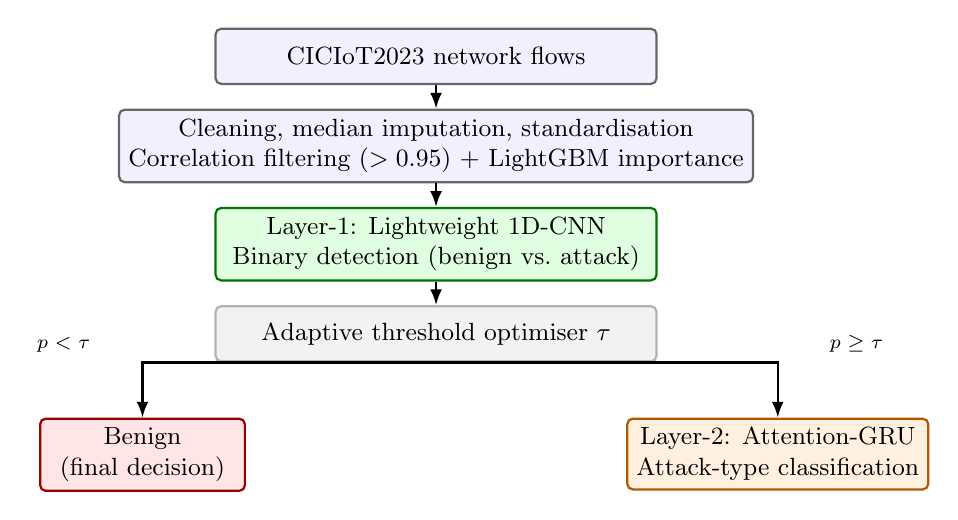
\begin{tikzpicture}[
  node distance=3mm and 8mm,
  box/.style={rectangle, rounded corners=2pt, draw=black!60, thick,
              minimum width=5.6cm, minimum height=0.7cm, align=center,
              font=\small, fill=blue!6},
  boxg/.style={box, fill=green!12, draw=green!45!black},
  boxr/.style={box, fill=red!10, draw=red!60!black, minimum width=2.6cm},
  boxo/.style={box, fill=orange!12, draw=orange!70!black, minimum width=2.6cm},
  arr/.style={-{Latex[length=2mm]}, thick}
]
\node[box] (data) {CICIoT2023 network flows};
\node[box, below=of data] (prep) {Cleaning, median imputation, standardisation\\ Correlation filtering ($>0.95$) + LightGBM importance};
\node[boxg, below=of prep] (cnn) {Layer-1: Lightweight 1D-CNN\\ Binary detection (benign vs.\ attack)};
\node[box, below=of cnn, fill=gray!10, draw=gray!60] (thr) {Adaptive threshold optimiser $\tau$};
\node[boxr, below left=7mm and -4mm of thr] (benign) {Benign\\ (final decision)};
\node[boxo, below right=7mm and -4mm of thr] (l2) {Layer-2: Attention-GRU\\ Attack-type classification};

\draw[arr] (data) -- (prep);
\draw[arr] (prep) -- (cnn);
\draw[arr] (cnn) -- (thr);
\draw[arr] (thr.south) -| (benign.north) node[midway, above, xshift=-10mm, font=\scriptsize] {$p< \tau$};
\draw[arr] (thr.south) -| (l2.north) node[midway, above, xshift=10mm, font=\scriptsize] {$p \geq \tau$};
\end{tikzpicture}
\caption{Overall HAGNet hierarchical intrusion detection framework.}
\label{fig:architecture}
\end{figure}

\subsection{Data Preprocessing and Feature Selection}

Prior to model training, raw CICIoT2023 flow records are cleaned by removing non-informative identifiers, converting infinite values to missing values, coercing attributes to numeric form, imputing missing values with the per-feature median, and standardising features to zero mean and unit variance. From the 80 remaining numerical features, a two-step pipeline is applied: (i) correlation-based filtering removes features with pairwise absolute correlation above 0.95; and (ii) a LightGBM~\cite{ref14} gradient-boosted tree ensemble is trained on the correlation-filtered pool, and its gain-based feature importance is used to retain the top 40 features. Mutual information between each feature and the target label was also evaluated during pipeline development, but the deployed feature set is the one ranked by LightGBM importance. This 40-dimensional vector is the shared input for both Layer-1 and Layer-2 models, lowering memory footprint and inference latency relative to the full 80-feature representation.

\subsection{Layer-1: Lightweight 1D-CNN Binary Detector}

The first stage of HAGNet is a compact 1D-CNN treating the 40-dimensional feature vector as a one-dimensional signal, applying convolutional filters to learn local interactions between adjacent, importance-ranked inputs. The network outputs the probability that a given flow is malicious:
\begin{equation}
P(y=1 \mid x) = \sigma(Wx + b),
\label{eq:binary}
\end{equation}
where $x$ denotes the learned convolutional feature representation, $W$ and $b$ are the weight matrix and bias of the output layer, and $\sigma(\cdot)$ is the sigmoid activation function. The architecture is intentionally shallow (Table~\ref{tab:cnn}, Section~\ref{sec:dataset}) so that it can be executed with low latency on the large volume of predominantly benign traffic that any deployed IDS must continuously process.

\subsection{Adaptive Threshold Optimisation and Routing}

Rather than committing to the conventional decision threshold of 0.5, HAGNet selects the operating threshold $\tau$ by sweeping candidate values over the validation set and choosing, among thresholds satisfying benign recall $\geq 0.60$ and attack recall $\geq 0.90$, the value that maximises macro-F1 (falling back to unconstrained macro-F1 maximisation if no threshold satisfies both constraints). This reflects the practical reality of network defence, where the cost of a missed attack (false negative) substantially exceeds the cost of a false alarm on benign traffic (false positive). The resulting routing rule is:
\begin{equation}
\hat{y} =
\begin{cases}
\text{Benign}, & p < \tau, \\
\text{Layer-2}, & p \geq \tau,
\end{cases}
\label{eq:routing}
\end{equation}
where $p = P(y=1\mid x)$ is the Layer-1 output probability. Flows routed to Layer-2 are those the system considers sufficiently likely to be malicious to warrant the additional computational cost of fine-grained categorisation.

\subsection{Layer-2: Attention-GRU Attack Classifier}

Flows routed by the threshold optimiser are passed to a second-stage classifier that identifies the specific attack family. This stage uses a GRU~\cite{ref12} to process the feature representation as a sequence of hidden states $h_1, \ldots, h_T$, followed by an additive attention mechanism~\cite{ref13} emphasising the most discriminative states rather than treating them uniformly. The attention weight assigned to hidden state $t$ is computed as
\begin{equation}
\alpha_t = \frac{\exp(e_t)}{\sum_{k=1}^{T} \exp(e_k)},
\label{eq:attention}
\end{equation}
where $e_t$ is a learned alignment score for hidden state $h_t$. The attention-weighted context vector is then obtained as
\begin{equation}
C = \sum_{t=1}^{T} \alpha_t h_t,
\label{eq:context}
\end{equation}
and is passed through a dense ReLU layer followed by a softmax output layer producing a probability distribution over attack categories. Because Layer-2 is only invoked for traffic already flagged malicious by Layer-1, its training set can be class-balanced (Section~\ref{sec:dataset}) without discarding benign samples, letting the attention mechanism learn attack-specific patterns without being overwhelmed by the benign class dominant in raw traffic.

\section{Dataset and Experimental Setup}
\label{sec:dataset}

\subsection{CICIoT2023 Dataset}

The proposed HAGNet framework is evaluated using the CICIoT2023 benchmark dataset~\cite{ref11}, one of the largest publicly available datasets for IoT intrusion detection, simulating realistic IoT environments with benign traffic and diverse cyberattacks generated from multiple smart devices and protocols. Compared with earlier datasets such as NSL-KDD~\cite{ref17} and CICIDS2017~\cite{ref18}, CICIoT2023 offers significantly larger traffic diversity and better represents modern IoT attack scenarios~\cite{ref9,ref10}.

For this study, six traffic categories were selected, comprising one benign class and five representative attack types. After merging all traffic flows, the final dataset contained 2{,}318{,}743 network instances with 80 numerical features following preprocessing (Table~\ref{tab:traffic}).

\begin{table}[!htb]
\centering
\caption{Traffic categories used in this study.}
\label{tab:traffic}
\small
\begin{tabular}{lrl}
\toprule
\textbf{Class} & \textbf{Samples} & \textbf{Type} \\
\midrule
Benign                  & 183{,}630   & Normal traffic \\
DoS-HTTP Flood          & 932{,}513   & DoS attack \\
Vulnerability Scan      & 869{,}923   & Reconnaissance \\
DDoS ACK Fragmentation  & 323{,}886   & DDoS attack \\
Mirai Greeth Flood      & 5{,}172     & Botnet \\
Dictionary Brute Force  & 3{,}619     & Credential attack \\
\midrule
\textbf{Total}          & \textbf{2{,}318{,}743} & --- \\
\bottomrule
\end{tabular}
\end{table}

The attack distribution is highly imbalanced, with DoS and Vulnerability Scan traffic dominating the dataset while Mirai and Dictionary Brute Force attacks contain relatively few samples, directly motivating the hierarchical learning strategy and class-balanced training adopted in Layer-2.

\subsection{Preprocessing, Data Split, and Experimental Configuration}

\textbf{Data cleaning.} Before model development, all traffic records underwent a structured preprocessing pipeline: removal of non-informative identifiers (flow ID, source/destination IP, original labels); conversion of infinite values to missing values; numeric conversion of all attributes; median imputation; and standard-scaler feature standardisation, producing a clean feature matrix suitable for deep neural network training.

\textbf{Training, validation and test split.} To ensure unbiased model evaluation, the dataset was divided using stratified sampling based on attack categories. A 70:15:15 split was adopted for training, validation, and testing, respectively (Table~\ref{tab:split}), preserving the class distribution across all subsets and preventing minority attack categories from disappearing during evaluation.

\textbf{Experimental configuration.} All experiments were implemented in Python using TensorFlow and Scikit-learn. The CNN and Attention-GRU models (Table~\ref{tab:hyperparams}) were trained independently using Adam with early stopping. Binary classification employed binary cross-entropy loss, while the multiclass attack classifier used sparse categorical cross-entropy. The binary detector receives the top 40 selected features, while the Attention-GRU processes only malicious traffic routed from Layer-1, avoiding unnecessary multiclass prediction on benign samples.

\begin{figure}[!htb]
\CenterFloatBoxes
\begin{floatrow}[2]
\ttabbox{%
\small
\begin{tabular}{lrr}
\toprule
\textbf{Subset} & \textbf{Samples} & \textbf{\%} \\
\midrule
Training   & 1{,}623{,}120 & 70\% \\
Validation & 347{,}811     & 15\% \\
Testing    & 347{,}812     & 15\% \\
\bottomrule
\end{tabular}}
{\caption{Dataset partition.}\label{tab:split}}
\ttabbox{%
\small
\begin{tabular}{lcc}
\toprule
\textbf{Param.} & \textbf{L1-CNN} & \textbf{L2-GRU} \\
\midrule
Input features    & 40      & 40 \\
Optimiser         & Adam    & Adam \\
Batch size        & 256     & 256 \\
Max.\ epochs      & 30      & 40 \\
Early stopping    & Pat.=3  & Pat.=3 \\
Output act.       & Sigmoid & Softmax \\
\bottomrule
\end{tabular}}
{\caption{Model hyperparameters.}\label{tab:hyperparams}}
\end{floatrow}
\end{figure}

\subsection{Evaluation Metrics and Class Imbalance Handling}

The performance of HAGNet is assessed using standard classification metrics derived from the confusion matrix. Let TP, TN, FP, and FN denote true positives, true negatives, false positives, and false negatives, respectively:
\begin{equation}
\text{Accuracy} = \frac{TP + TN}{TP + TN + FP + FN}, \qquad
\text{Precision} = \frac{TP}{TP + FP},
\end{equation}
\begin{equation}
\text{Recall} = \frac{TP}{TP + FN}, \qquad
F1 = 2 \times \frac{\text{Precision} \times \text{Recall}}{\text{Precision} + \text{Recall}}.
\end{equation}
For Layer-1, additional emphasis is placed on attack recall and balanced accuracy, since missing malicious traffic poses a greater security risk than incorrectly flagging benign traffic; the threshold satisfying the predefined security constraint (Section~\ref{sec:methodology}) is selected for deployment. The malicious attack classes also exhibit substantial imbalance, particularly for the Mirai and Dictionary Brute Force categories. Rather than oversampling the entire dataset, balancing is performed only for Layer-2 attack classification: minority classes are resampled to match the largest attack category, creating a balanced training distribution while preserving the original validation and test sets, enabling the Attention-GRU to learn equally from all attack categories without biasing the evaluation. Effective-number-based class re-weighting~\cite{ref15} was also evaluated as an alternative to resampling during development, but per-class oversampling was retained as it gave more consistent class exposure within each mini-batch.

\section{Results and Discussion}
\label{sec:results}

\subsection{Layer-1 Binary Intrusion Detection}

The proposed HAGNet framework is evaluated on the CICIoT2023 held-out test set in two sequential stages: Layer-1 binary intrusion detection and Layer-2 attack classification. The hierarchical routing mechanism ensures that only malicious traffic is processed by the Attention-GRU classifier, reducing computational overhead while maintaining high detection performance. The first stage distinguishes benign and malicious traffic using the lightweight 1D-CNN described in Table~\ref{tab:cnn}. Instead of using the conventional decision threshold of 0.5, the threshold is optimised over the validation set by maximising macro-F1 subject to the security constraints defined in Section~\ref{sec:methodology} (benign recall $\geq 0.60$, attack recall $\geq 0.90$), as illustrated schematically in Figure~\ref{fig:threshold}.

\begin{figure}[!htb]
\CenterFloatBoxes
\begin{floatrow}[2]
\ttabbox{%
\small
\begin{tabular}{ll}
\toprule
\textbf{Layer} & \textbf{Config.} \\
\midrule
Input                   & $40 \times 1$ \\
Conv1D                  & 16 filt., $k$=3, same \\
Batch Norm.             & Yes \\
Conv1D                  & 32 filt., $k$=3, same \\
Glob.\ Avg.\ Pooling    & 1D \\
Dense                   & 16 neurons \\
Output                  & Sigmoid \\
\bottomrule
\end{tabular}}
{\caption{Layer-1 CNN architecture.}\label{tab:cnn}}
\ffigbox{%
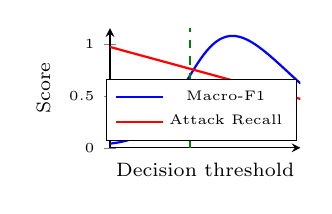
\begin{tikzpicture}
\begin{axis}[
  width=4.0cm, height=3.1cm,
  xlabel={\scriptsize Decision threshold}, ylabel={\scriptsize Score},
  xmin=0, xmax=1, ymin=0, ymax=1.15,
  xtick=\empty, ytick={0,0.5,1}, tick label style={font=\tiny},
  legend style={font=\tiny, at={(0.98,0.06)}, anchor=south east},
  axis lines=left,
]
\addplot[thick, blue, domain=0:1, samples=60] {1/(1+exp(-9*(x-0.42))) * exp(-2.4*(x-0.42)^2) *1.35 + 0.02};
\addlegendentry{Macro-F1}
\addplot[thick, red, domain=0:1, samples=60] {0.97 - 0.5*x};
\addlegendentry{Attack Recall}
\draw[dashed, green!50!black, thick] (axis cs:0.42,0) -- (axis cs:0.42,1.15);
\node[font=\tiny, green!40!black, align=left] at (axis cs:0.42,1.28) {Selected $\tau$};
\end{axis}
\end{tikzpicture}}
{\caption{Optimal routing threshold $\tau$: macro-F1 vs.\ attack recall.}\label{fig:threshold}}
\end{floatrow}
\end{figure}

Table~\ref{tab:layer1-results} contrasts Layer-1 performance at a low, unoptimised initial threshold (0.05) against the optimised threshold $\tau$. At the low threshold, the model over-flags benign traffic (benign recall only 0.53; confusion matrix $\begin{pmatrix} 14{,}676 & 12{,}869 \\ 613 & 49{,}575 \end{pmatrix}$, ordered Benign/Attack), giving 83\% accuracy. Optimising $\tau$ raises benign recall to 0.97 while attack recall falls only slightly, from 0.99 to 0.94, cutting false positives by 94\% (12{,}869 $\to$ 722) at the cost of 2{,}433 additional false negatives (613 $\to$ 3{,}046); confusion matrix $\begin{pmatrix} 26{,}823 & 722 \\ 3{,}046 & 47{,}142 \end{pmatrix}$. Overall accuracy rises from 83\% to 95\%, and macro-F1 from 0.78 to 0.95, confirming that threshold optimisation is essential rather than incidental to this architecture.

\begin{table}[!htb]
\centering
\caption{Layer-1 binary detection performance on the CICIoT2023 test set, before and after threshold optimisation (support: Benign 27{,}545; Attack 50{,}188; total 77{,}733).}
\label{tab:layer1-results}
\small
\begin{tabular}{lcccccc}
\toprule
& \multicolumn{3}{c}{\textbf{Threshold = 0.05}} & \multicolumn{3}{c}{\textbf{Optimised $\tau$}} \\
\cmidrule(lr){2-4}\cmidrule(lr){5-7}
\textbf{Class} & P & R & F1 & P & R & F1 \\
\midrule
Benign          & 0.96 & 0.53 & 0.69 & 0.90 & 0.97 & 0.93 \\
Attack          & 0.79 & 0.99 & 0.88 & 0.98 & 0.94 & 0.96 \\
\midrule
Accuracy        & \multicolumn{3}{c}{0.83} & \multicolumn{3}{c}{0.95} \\
Macro avg       & 0.88 & 0.76 & 0.78 & 0.94 & 0.96 & 0.95 \\
Weighted avg    & 0.85 & 0.83 & 0.81 & 0.95 & 0.95 & 0.95 \\
\bottomrule
\end{tabular}
\end{table}

\subsection{Layer-2 Attack Classification}

After binary screening, only malicious traffic is forwarded to the Attention-GRU model (Table~\ref{tab:gru}, Figure~\ref{fig:gru}) for fine-grained attack categorisation. The second stage receives balanced malicious samples through class-aware resampling, reducing the influence of the severe class imbalance present in the original dataset. The attention mechanism assigns adaptive importance weights to informative temporal representations, allowing the GRU to focus on discriminative attack characteristics rather than treating all features equally.

\begin{table}[!htb]
\centering
\caption{Attention-GRU configuration.}
\label{tab:gru}
\small
\begin{tabular}{ll}
\toprule
\textbf{Parameter} & \textbf{Value} \\
\midrule
Input features   & 40 \\
GRU units        & 32 \\
Attention layer  & Dense + Softmax \\
Dense layer      & 16 neurons \\
Output           & Softmax \\
Optimiser        & Adam \\
\bottomrule
\end{tabular}
\end{table}

\begin{figure}[!htb]
\centering
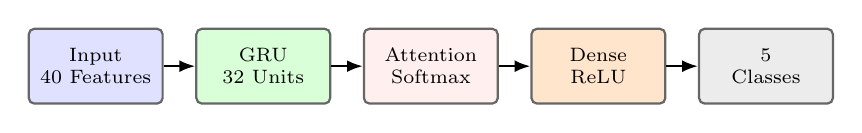
\begin{tikzpicture}[
  node distance=4mm,
  box/.style={rectangle, rounded corners=2pt, draw=black!60, thick,
              minimum width=1.7cm, minimum height=0.95cm, align=center, font=\scriptsize},
  arr/.style={-{Latex[length=2mm]}, thick}
]
\node[box, fill=blue!12]   (in)   {Input\\40 Features};
\node[box, fill=green!15, right=of in]  (gru)  {GRU\\32 Units};
\node[box, fill=pink!25, right=of gru] (att)  {Attention\\Softmax};
\node[box, fill=orange!20, right=of att] (dense){Dense\\ReLU};
\node[box, fill=gray!15, right=of dense] (out) {5\\Classes};
\draw[arr] (in) -- (gru);
\draw[arr] (gru) -- (att);
\draw[arr] (att) -- (dense);
\draw[arr] (dense) -- (out);
\end{tikzpicture}
\caption{Architecture of the Layer-2 Attention-GRU attack classifier.}
\label{fig:gru}
\end{figure}

Table~\ref{tab:layer2-results} reports per-class Layer-2 performance on the 47{,}142 test attacks that Layer-1 correctly routed as malicious. The Attention-GRU attains 97.2\% accuracy on this subset (macro-F1 $=0.756$, weighted F1 $=0.975$); the dominant classes (DDoS-ACK Fragmentation, DoS-HTTP Flood) are classified almost perfectly (F1 $\geq 0.976$), while the rarest classes (Mirai Greeth Flood, Dictionary Brute Force) retain high recall (0.67--0.97) from class-balanced training but low precision (0.27--0.30), since a small absolute number of misrouted majority-class flows disproportionately dilutes precision for classes with only 120--195 test instances.

\begin{table}[!htb]
\centering
\caption{Layer-2 per-class attack classification performance.}
\label{tab:layer2-results}
\small
\begin{tabular}{lcccc}
\toprule
\textbf{Attack category} & \textbf{Precision} & \textbf{Recall} & \textbf{F1-score} & \textbf{Support} \\
\midrule
DDoS-ACK Fragmentation  & 0.996 & 0.986 & 0.991 & 18{,}978 \\
Dictionary Brute Force  & 0.303 & 0.967 & 0.461 & 120 \\
DoS-HTTP Flood          & 0.982 & 0.971 & 0.976 & 17{,}516 \\
Mirai Greeth Flood      & 0.272 & 0.672 & 0.387 & 195 \\
Vulnerability Scan      & 0.970 & 0.954 & 0.962 & 10{,}333 \\
\midrule
Accuracy                & \multicolumn{3}{c}{0.972} & 47{,}142 \\
Macro average           & 0.705 & 0.910 & 0.756 & 47{,}142 \\
Weighted average        & 0.980 & 0.972 & 0.975 & 47{,}142 \\
\bottomrule
\end{tabular}
\end{table}

\begin{table}[!htb]
\centering
\caption{Layer-2 confusion matrix (rows: true label, columns: predicted label). DBF = Dictionary Brute Force.}
\label{tab:layer2-cm}
\footnotesize
\begin{tabular}{lccccc}
\toprule
 & \textbf{DDoS} & \textbf{DBF} & \textbf{DoS-HTTP} & \textbf{Mirai} & \textbf{VulnScan} \\
\midrule
DDoS-ACK Frag.  & 18{,}712 & 25  & 119    & 97  & 25    \\
DBF             & 0        & 116 & 2      & 1   & 1     \\
DoS-HTTP Flood  & 72       & 37  & 17{,}014 & 131 & 262   \\
Mirai Greeth    & 1        & 19  & 29     & 131 & 15    \\
VulnScan        & 0        & 186 & 169    & 122 & 9{,}856 \\
\bottomrule
\end{tabular}
\end{table}

\subsection{Comparative Analysis and Discussion}

The proposed hierarchical framework addresses several limitations of existing IoT intrusion detection models. Unlike conventional CNN or GRU models that perform direct multiclass classification, HAGNet separates anomaly detection and attack recognition into two specialised stages. Table~\ref{tab:qualitative} compares HAGNet against representative model families along four design axes.

\begin{table}[!htb]
\centering
\caption{Qualitative comparison with existing model families.}
\label{tab:qualitative}
\small
\begin{tabular}{lcccc}
\toprule
\textbf{Model} & \textbf{Binary Screening} & \textbf{Attention} & \textbf{Hierarchical} & \textbf{Edge Suitable} \\
\midrule
CNN            & \ding{55} & \ding{55}    & \ding{55} & \ding{51} \\
LSTM           & \ding{55} & \ding{55}    & \ding{55} & \ding{55} \\
CNN--GRU       & \ding{55} & Limited      & \ding{55} & Moderate \\
Transformer IDS& \ding{55} & \ding{51}    & \ding{55} & \ding{55} \\
\textbf{HAGNet}& \ding{51} & \ding{51}    & \ding{51} & \ding{51} \\
\bottomrule
\end{tabular}
\end{table}

Recent hybrid CNN--GRU models show strong performance for IoT intrusion detection, while surveys emphasise hierarchical learning and lightweight deployment as future directions~\cite{ref6,ref7,ref4}, both of which HAGNet integrates.

Decomposing intrusion detection into two sequential tasks offers practical advantages over flat multiclass architectures. The Layer-1 CNN rapidly filters benign traffic with a lightweight model; the Attention-GRU then focuses exclusively on malicious traffic, reducing the effect of class imbalance; and adaptive threshold optimisation prioritises attack recall instead of an arbitrary probability threshold.

These characteristics collectively improve the scalability of HAGNet for real-time IoT intrusion detection, particularly in edge-enabled cyber-physical systems where computational efficiency is as important as detection accuracy. The results in Tables~\ref{tab:layer1-results} and~\ref{tab:layer2-results} correspond to a single training run with a fixed random seed; reporting confidence intervals across multiple seeds is left as a direction for more extensive validation.

\section{Conclusion and Future Work}
\label{sec:conclusion}

This paper presented HAGNet (Hierarchical Attention-GRU Network), a two-stage deep learning framework for intelligent IoT intrusion detection using network flow features from the CICIoT2023 dataset. Unlike conventional flat multiclass intrusion detection systems, the proposed framework decomposes detection into binary anomaly detection followed by fine-grained attack categorisation, enabling each model to specialise in a simpler objective. The complete framework integrates data preprocessing, correlation-based feature reduction, LightGBM gain-based feature selection, a lightweight 1D-CNN for malicious traffic screening, adaptive threshold optimisation, and an Attention-based GRU for attack classification. On the held-out test set, HAGNet achieves 95\% Layer-1 accuracy with 94\% attack recall, and 97.2\% Layer-2 accuracy on correctly-routed attacks, though minority attack families remain harder to classify with high precision.

The hierarchical routing strategy reduces overhead by forwarding only malicious traffic to the second-stage classifier, suiting edge-enabled IoT environments. Adaptive threshold optimisation further prioritises security-sensitive detection over a fixed threshold, addressing limitations including class imbalance, inter-class confusion, and the lack of scalable hierarchical IDS architectures~\cite{ref1,ref2,ref5}. Overall, HAGNet shows that lightweight binary screening, attention-guided temporal learning, and adaptive routing offer a scalable direction for next-generation IoT intrusion detection.

\noindent\textbf{Future work.} Several directions can further enhance the framework's practical applicability:
\begin{itemize}
    \item \textbf{Transformer-based sequential learning:} replace the GRU with a lightweight Transformer~\cite{ref20} or temporal-attention model for long-range dependencies~\cite{ref4}.
    \item \textbf{Federated intrusion detection:} a privacy-preserving federated HAGNet, following the federated averaging paradigm~\cite{ref21}, enabling collaborative learning across distributed IoT devices without sharing raw traffic~\cite{ref3}.
    \item \textbf{Explainable AI integration:} SHAP~\cite{ref22} or attention-visualisation to assist analysts in interpreting attack decisions.
    \item \textbf{Real-time edge deployment:} optimise the CNN for hardware such as Raspberry Pi, NVIDIA Jetson, or TinyML accelerators.
    \item \textbf{Generalised attack detection:} extend the framework to zero-day attacks via self-supervised or continual learning.
\end{itemize}
These extensions would improve the robustness and deployment readiness of hierarchical IDS for future IoT infrastructures.

\begin{thebibliography}{22}
\setlength{\itemsep}{-2pt}

\bibitem{ref1}
Al-Hawawreh, M., Sitnikova, E.: Intelligent approaches toward intrusion detection systems for industrial internet of things: a systematic comprehensive review. J. Netw. Comput. Appl. \textbf{215}, 103444 (2023)

\bibitem{ref2}
A comprehensive survey of intrusion detection systems in IoT: datasets, algorithms, and emerging trends. Appl. Comput. Intell. Soft Comput. \textbf{2026}, 5545578 (2026)

\bibitem{ref3}
Saied, M., Guirguis, S., Madbouly, M.: Review of artificial intelligence for enhancing intrusion detection in the internet of things. Eng. Appl. Artif. Intell. \textbf{127}, 107231 (2024)

\bibitem{ref4}
Aldhaheri, A., Alwahedi, F., Ferrag, M.A., Battah, A.: Deep learning for cyber threat detection in IoT networks: a review. Internet Things Cyber-Phys. Syst. \textbf{4}, 110--128 (2024)

\bibitem{ref5}
Sagu, A., Gill, N.S., Gulia, P., Alduaiji, N., Shukla, P.K., Shah, M.A.: Advances to IoT security using a GRU-CNN deep learning model trained on SUCMO algorithm. Sci. Rep. \textbf{15}, 99574 (2025)

\bibitem{ref6}
Ghosh, K.P., Hasan, M., Robin, M.T.I., Hossain, M.A., Islam, M.S.: A novel deep learning framework with temporal attention convolutional networks for intrusion detection in IoT and IIoT networks. Sci. Rep. \textbf{15}, 32697 (2025)

\bibitem{ref7}
Cevallos Moreno, J.F., Rizzardi, A., Sicari, S., Coen-Porisini, A.: Deep reinforcement learning for intrusion detection in Internet of Things: best practices, lessons learnt, and open challenges. Comput. Netw. \textbf{236}, 110016 (2023)

\bibitem{ref9}
Meziane, H., Ouerdi, N.: A survey on performance evaluation of artificial intelligence algorithms for improving IoT security systems. Sci. Rep. \textbf{13}, 21255 (2023)

\bibitem{ref10}
Intrusion detection in the Internet of Things: a comprehensive review of techniques, architectures, datasets, and emerging trends. Sensors \textbf{26}(11), 3405 (2026)

\bibitem{ref11}
Neto, E.C.P., Dadkhah, S., Ferreira, R., Zohourian, A., Lu, R., Ghorbani, A.A.: CICIoT2023: a real-time dataset and benchmark for large-scale attacks in IoT environment. Sensors \textbf{23}(13), 5941 (2023)

\bibitem{ref12}
Cho, K., van Merri\"enboer, B., Gulcehre, C., Bahdanau, D., Bougares, F., Schwenk, H., Bengio, Y.: Learning phrase representations using RNN encoder-decoder for statistical machine translation. In: Proc. EMNLP, pp.\ 1724--1734 (2014)

\bibitem{ref13}
Bahdanau, D., Cho, K., Bengio, Y.: Neural machine translation by jointly learning to align and translate. In: Proc. ICLR (2015)

\bibitem{ref14}
Ke, G., Meng, Q., Finley, T., Wang, T., Chen, W., Ma, W., Ye, Q., Liu, T.Y.: LightGBM: a highly efficient gradient boosting decision tree. In: Advances in Neural Information Processing Systems 30 (NeurIPS), pp.\ 3146--3154 (2017)

\bibitem{ref15}
Cui, Y., Jia, M., Lin, T.Y., Song, Y., Belongie, S.: Class-balanced loss based on effective number of samples. In: Proc. IEEE/CVF CVPR, pp.\ 9268--9277 (2019)

\bibitem{ref17}
Tavallaee, M., Bagheri, E., Lu, W., Ghorbani, A.A.: A detailed analysis of the KDD CUP 99 data set. In: Proc. IEEE Symp.\ Computational Intelligence for Security and Defense Applications (CISDA), pp.\ 1--6 (2009)

\bibitem{ref18}
Sharafaldin, I., Lashkari, A.H., Ghorbani, A.A.: Toward generating a new intrusion detection dataset and intrusion traffic characterization. In: Proc. ICISSP, pp.\ 108--116 (2018)

\bibitem{ref19}
Koroniotis, N., Moustafa, N., Sitnikova, E., Turnbull, B.: Towards the development of realistic botnet dataset in the Internet of Things for network forensic analytics: Bot-IoT dataset. Future Gener.\ Comput.\ Syst. \textbf{100}, 779--796 (2019)

\bibitem{ref20}
Vaswani, A., Shazeer, N., Parmar, N., Uszkoreit, J., Jones, L., Gomez, A.N., Kaiser, {\L}., Polosukhin, I.: Attention is all you need. In: Advances in Neural Information Processing Systems 30 (NeurIPS), pp.\ 5998--6008 (2017)

\bibitem{ref21}
McMahan, B., Moore, E., Ramage, D., Hampson, S., y Arcas, B.A.: Communication-efficient learning of deep networks from decentralized data. In: Proc. AISTATS, pp.\ 1273--1282 (2017)

\bibitem{ref22}
Lundberg, S.M., Lee, S.I.: A unified approach to interpreting model predictions. In: Advances in Neural Information Processing Systems 30 (NeurIPS), pp.\ 4765--4774 (2017)

\end{thebibliography}

\end{document}
